%!TEX encoding = UTF-8 Unicode
%!TEX program = xelatex

\documentclass[bachelor]{ustcthesis}
% bachelor|master|doctor
\usepackage{float}
\usepackage{listings}
\usepackage{ustcextra}
\graphicspath{{figures/}}
\bibliographystyle{ustcauthoryear}
% \bibliographystyle{ustcnumerical}

\renewpagestyle{front}[\zihao{-5}]{
    \sethead{}{软件工程作业管理系统概要设计}{}
    \setfoot{}{\thepage}{}
    \headrule
}
\renewpagestyle{main}[\zihao{-5}]{
    \sethead{}{软件工程作业管理系统概要设计}{}
    \setfoot{}{\thepage}{}
    \headrule
}
\newcommand{\HRule}{\rule{\linewidth}{0.5mm}}
\newcommand{\tabincell}[2]{\begin{tabular}{@{}#1@{}}#2\end{tabular}}

\begin{document}



\begin{titlepage}
\begin{center}
~\\[5cm]
\HRule \\[0.4cm]
{\huge \bfseries 软件工程作业管理系统\\概要设计}\\[0.4cm]
\HRule \\[1.5cm]

\begin{tabular}{ccc}
  & 人员 & 日期 \\ 
拟制 & 张三\ 李四\ 王五 & yyyy-mm-dd \\ 
评审人 & • & yyyy-mm-dd \\ 
批准 & • & yyyy-mm-dd \\ 
签发 & • & yyyy-mm-dd \\ 
\end{tabular} 

\end{center}
\end{titlepage}



\frontmatter
\begin{abstract}
	本文是关于一款云播放器的概要设计文档,内容包括云播放器的任务概述、总体设计、接口设计、数据结构设计、数据库设计、界面设计、出错处理设计和维护设计等详细描述。在于为开发和维护人员提供参考手册。本文档的预期读者为系统设计人员、软件开发人员、客户方的系统设计人员和项目评审人员。
	
	
	\keywords{云播放器\zhspace{}需求规格说明\zhspace{} 云音乐\zhspace{} 软件工程\zhspace{}说明文档}
	
	\begin{table}[htbp]
		\centering
		\caption{缩略词清单} \label{tab:abbr}
		\begin{tabular}{|c|c|c|}
			\hline
			缩略语 & 英文全名 & 中文解释 \\
			\hline
			SDK& Software Development Kit & 软件开发工具包\\
			ADK& Android Open Accessory Development Kit &Android开放配件开发工具包\\
			DB &DataBase&数据库\\
			DBA &Database administration&数据库管理员\\
			UI &User Interface&用户接口\\
			GUI &Graphic User Interface&图形化用户界面\\
			
			\hline
		\end{tabular}
	\end{table}
	
\end{abstract}

\tableofcontents
\listoffigures
\listoftables
% \listofalgorithms  % 算法索引,如不需要,可直接注释掉本行
% \begin{notation}

%\centering
%XX 软件需求规格说明书

%关键词:能够体现文档描述内容主要方面的词汇。
 
%摘要:


\centering
\begin{tabular}{rl}
$\ln x$ & natural logarithm $\log_ex$ \\
$\log x$ & common logarithm $\log_{10}x$ \\
$x\ \mathrm{mod}\ y$ & remainder \\
\end{tabular}

\end{notation}


\mainmatter
\chapter{引言}
\section{编写目的}
在本项目的前一阶段,也就是需求分析阶段,已经将系统用户对本系统的需求做了详细的阐述,这些用户需求已经在上一阶段中对不同用户所提出的不同功能,实现的各种效果做了调研工作,并在需求规格说明书中得到详尽得叙述及阐明。

本阶段已在系统的需求分析的基础上,对即时聊天工具做概要设计。主要解决了实现该系统需求的程序模块设计问题。包括如何把该系统划分成若干个模块、决定各个模块之间的接口、模块之间传递的信息,以及数据结构、模块结构的设计等。在以下的概要设计报告中将对在本阶段中对系统所做的所有概要设计进行详细的说明,在设计过程中起到了提纲挈领的作用。

在下一阶段的详细设计中,程序设计员可参考此概要设计报告,在概要设计即时聊天工具所做的模块结构设计的基础上,对系统进行详细设计。在以后的软件测试以及软件维护阶段也可参考此说明书,以便于了解在概要设计过程中所完成的各模块设计结构,或在修改时找出在本阶段设计的不足或错误。


\section{项目背景}
随着互联网的快速发展和网速的不断提高,互联网用户的音乐需求已不再是单单的购买专辑并用专门的播放设备进行播放.他们更需要随时随地都能够收听到自己喜爱的歌曲,利用网络,而不是本地实体进行音乐的欣赏.同时,用户也迫切的希望能够定义一个属于自己的歌曲列表,并能够随时访问并更新.智能手机的产生为用户这一需求的满足提供了条件,本项目依托于云端存储和手机智能系统,为用户提供音乐点播功能,并允许用户自定义歌曲列表,以满足不同人群的风格需求.

\section{术语}
[列出本文档中所用到的专门术语的定义和外文缩写的原词组]
\begin{table}[htbp]
\centering
\caption{术语表} \label{tab:terminology}
\begin{tabular}{|c|c|}
    \hline
    缩写、术语 & 解释 \\
    \hline
    SQL & SQL 指结构化查询语言,使我们有能力访问数据库 \\
    \hline
\end{tabular}
% \note{这里是表的注释}
\end{table}
\chapter{任务概述}
本系统的目标是实现一个云音乐播放系统,包括客户端、服务器端两个部分。

客户端面向个人用户,为用户提供音乐播放、音乐管理和音乐推荐服务。

\section{目标}
实现云音乐播放系统系统,实现需求规格说明书中所描述的
歌曲播放 (本地/在线)功能、
歌曲搜索功能、
歌单创建与收藏功能、
关联推荐、
每日推荐歌单、
用户个人信息管理 (登录, 注册, 信息更改)功能
并且保证系统的健壮性和数据安全。

\section{开发与运行环境}

\subsection{开发环境的配置}
\begin{table}[htbp]
	\centering
	\caption{开发环境的配置} \label{tab:development-environment}
	\begin{tabular}{|c|c|c|}
		\hline
		类别 & 标准配置 & 最低配置 \\
		\hline
		计算机硬件 & \tabincell{c}{基于x86结构的CPU\\ 主频>=2.4GHz\\ 内存>=8G\\ 硬盘>=200G } & \tabincell{c}{基于x86结构的CPU\\ 主频>=1.6GHz\\ 内存>=512M\\ 硬盘>=2G} \\
		\hline
		计算机软件 & \tabincell{c}{Linux (kernel version>=4.10)\\ GNU gcc (version>=6.3.1)\\Android Studio 2.3.1 } & \tabincell{c}{Linux (kernel version>=3.10)\\ GNU gcc (version>=5.4\\Android Studio 2.3.1} \\
		\hline
		网络通信 & \tabincell{c}{至少要有一块可用网卡\\ 能运行IP协议栈即可} & \tabincell{c}{至少要有一块可用网卡\\ 能运行IP协议栈即可} \\
		\hline
		其他 & \tabincell{c}{采用 MySQL 数据库\\ 使用git进行版本控制} & \tabincell{c}{采用 MySQL 数据库\\ 使用git进行版本控制} \\
		\hline
	\end{tabular}
	% \note{这里是表的注释}
\end{table}

\subsection{测试环境的配置}
\begin{table}[htbp]
	\centering
	\caption{服务器端测试环境的配置} \label{tab:test-environment}
	\begin{tabular}{|c|c|c|}
		\hline
		类别 & 标准配置 & 最低配置 \\
		\hline
		计算机硬件 & \tabincell{c}{基于x86结构的CPU\\ 主频>=2.4GHz\\ 内存>=8G\\ 硬盘>=200G } & \tabincell{c}{基于x86结构的CPU\\ 主频>=1.6GHz\\ 内存>=512M\\ 硬盘>=2G} \\
		\hline
		计算机软件 & \tabincell{c}{Linux (kernel version>=4.10)\\ GNU gcc (version>=6.3.1)\\Android Studio 2.3.1 } & \tabincell{c}{Linux (kernel version>=3.10)\\ GNU gcc (version>=5.4)\\Android Studio 2.3.1} \\
		\hline
		网络通信 & \tabincell{c}{至少要有一块可用网卡\\ 能运行IP协议栈即可} & \tabincell{c}{至少要有一块可用网卡\\ 能运行IP协议栈即可} \\
		\hline
		其他 & \tabincell{c}{采用 MySQL 数据库\\ 使用git进行版本控制} & \tabincell{c}{采用 MySQL 数据库\\ 使用git进行版本控制} \\
		\hline
	\end{tabular}
	% \note{这里是表的注释}
\end{table}

\begin{table}[htbp]
	\centering
	\caption{客户端测试环境的配置} \label{tab:test-environment}
	\begin{tabular}{|c|c|c|}
		\hline
		类别 & 标准配置 & 最低配置 \\
		\hline
		计算机硬件 & \tabincell{c}{基于ARM结构的CPU\\ 主频>=2.0GHz\\ 内存>=2G\\ 硬盘>=16G} & \tabincell{c}{基于ARM结构的CPU\\ 主频>=1.6GHz\\ 内存>=1M\\ 硬盘>=2G} \\
		\hline
		计算机软件 & \tabincell{c}{Android (version>=6.1)\\ Android Studio 2.3.1 } & \tabincell{c}{Android (version>=4.1)\\ Android Studio 2.3.1 } \\
		\hline
		网络通信 & \tabincell{c}{至少要有一块可用网卡\\ 能运行IP协议栈即可} & \tabincell{c}{至少要有一块可用网卡\\ 能运行IP协议栈即可} \\
		\hline
		其他 & \tabincell{c}{能进行音乐播放} & \tabincell{c}{能进行音乐播放} \\
		\hline
	\end{tabular}
	% \note{这里是表的注释}
\end{table}


\subsection{运行环境的配置}
\begin{table}[htbp]
	\centering
	\caption{服务器端测试环境的配置} \label{tab:test-environment}
	\begin{tabular}{|c|c|c|}
		\hline
		类别 & 标准配置 & 最低配置 \\
		\hline
		计算机硬件 & \tabincell{c}{基于x86结构的CPU\\ 主频>=2.4GHz\\ 内存>=8G\\ 硬盘>=200G } & \tabincell{c}{基于x86结构的CPU\\ 主频>=1.6GHz\\ 内存>=512M\\ 硬盘>=2G} \\
		\hline
		计算机软件 & \tabincell{c}{Linux (kernel version>=4.10)\\ GNU gcc (version>=6.3.1)\\Android Studio 2.3.1 } & \tabincell{c}{Linux (kernel version>=3.10)\\ GNU gcc (version>=5.4)\\Android Studio 2.3.1} \\
		\hline
		网络通信 & \tabincell{c}{至少要有一块可用网卡\\ 能运行IP协议栈即可} & \tabincell{c}{至少要有一块可用网卡\\ 能运行IP协议栈即可} \\
		\hline
		其他 & \tabincell{c}{采用 MySQL 数据库\\ 使用git进行版本控制} & \tabincell{c}{采用 MySQL 数据库\\ 使用git进行版本控制} \\
		\hline
	\end{tabular}
	% \note{这里是表的注释}
\end{table}

\begin{table}[htbp]
	\centering
	\caption{客户端测试环境的配置} \label{tab:test-environment}
	\begin{tabular}{|c|c|c|}
		\hline
		类别 & 标准配置 & 最低配置 \\
		\hline
		计算机硬件 & \tabincell{c}{基于ARM结构的CPU\\ 主频>=2.0GHz\\ 内存>=2G\\ 硬盘>=16G} & \tabincell{c}{基于ARM结构的CPU\\ 主频>=1.6GHz\\ 内存>=1M\\ 硬盘>=2G} \\
		\hline
		计算机软件 & \tabincell{c}{Android (version>=6.1) } & \tabincell{c}{Android (version>=4.1) } \\
		\hline
		网络通信 & \tabincell{c}{至少要有一块可用网卡\\ 能运行IP协议栈即可} & \tabincell{c}{至少要有一块可用网卡\\ 能运行IP协议栈即可} \\
		\hline
		其他 & \tabincell{c}{能进行音乐播放} & \tabincell{c}{能进行音乐播放} \\
		\hline
	\end{tabular}
	% \note{这里是表的注释}
\end{table}

\section{需求概述}
功能需求包括:

\subsection{R.INTF.CLD.001 搜索}
\paragraph{介绍}
用户可以通过搜索框向云端发出搜索请求,云端从曲库中搜索相关歌曲,专辑,歌单,歌手信息,分别整理为列表并返回给本地客户端.

\paragraph{输入}

输入来源:本地客户端

输入格式:Unicode字符串

有效输入范围:1-99个字符

\paragraph{处理}

输入的有效性检测:搜索字符串应为长度为1-99的Unicode字符串


操作时序:
\begin{enumerate}
	\item 用户在搜索框内键入搜索字符串
	\item 用户点击搜索按钮向云端提交搜索请求
	\item 云端对搜索字符串进行验证,确定其是合法字符串
	\item 云端在歌曲,专辑,歌手,歌单 数据库中分别应用字符串进行搜索并整理成列表
	\item 云端将结果发回至客户端
	\item 客户端收到结果后,将其以合适的形式显示到屏幕上
\end{enumerate}

异常处理:
\begin{enumerate}
	\item 客户端输入框内字符串不合法:点击搜索按钮时客户端报告不合法输入,不发出搜索请求
	\item 云端接收到的字符串不合法:使搜索结果为空并返回到客户端
	\item 云端和本地通信失败:客户端提示失败原因,并进行收到空的结果的行为
\end{enumerate}


使用方法:

对数据库内执行搜索的算法:模糊搜索(待定)




\paragraph{输出}

从云端到本地:

输出位置:客户端请求接收器
输出数量:4
输出单位:信息列表
具体描述:4个信息列表分别信息单位为歌曲,专辑,歌手,歌单

从结果到屏幕:
输出位置:客户端屏幕
输出数量:4
具体描述:客户端通过选择结果标签页确定要显示歌曲,专辑,歌手,歌单的其中一个列表

\subsection{R.INTF.CLD.002 播放歌曲}

\paragraph{介绍}

播放是云音乐系统的最基本功能,用户通过选中界面上的一个歌曲项,即可播放相应歌曲.音乐文件的存储位置有本地和云端两个选项,用户可以通过下载功能来将云端的音乐文件下载到本地,在播放时将直接播放本地的歌曲.如果音乐文件不在本地,则云端通过流媒体的形式返回给客户端一个流,客户端再播放这个流.

\paragraph{输入}

输入来源:客户端

输入内容:一个歌曲项

用户选中界面上的一个歌曲项,歌曲项是客户端歌曲组织的基本形式,用户可以直接点击歌曲项来执行播放功能.用户可以从歌曲项获得歌曲的名称,歌手,所属专辑等信息.歌曲项还包含了一个独一无二的编码用来区分并永久性保存.事实上,发送到云端的一个播放请求可以仅是这个编码

\paragraph{处理}

有效性检测:

有效性的检测包含两个方面:本地和云端,本地的有效性检测优先于云端并是一个短路操作.如果在本地,歌曲被验证是有效的,即歌曲已在本地,则直接播放,不与云端交互.当本地无法验证有效性时,云端将检测请求播放的曲目是否有效,在本系统中等价于歌曲是否在云端曲库中,如果不在,播放请求无效.否则,认定播放请求有效.

操作时序:
\begin{enumerate}
	\item 用户点击客户端的歌曲项进行播放操作
	\item 系统生成播放请求,并在本地检测请求对应的歌曲是否在本地,如果在,直接播放该歌曲并进行相应状态的更新.否则,进入下一步.
	\item 客户端向云端发出请求,云端接收请求后检查该请求是否合法,如果不合法,向本地发回不合法原因.否则,云端创建一个流返回给客户端.
	\item 客户端接收到云端发来的流,进行播放,并进行相应状态的更新.
\end{enumerate}


异常处理:
\begin{enumerate}
	\item 云端不存在请求歌曲(请求不合法):向客户端发回不合法回应,指出该歌曲不存在
	\item 播放流时网络中断:播放进行到已缓存的最后位置停止,显示"网络已中断"信息
\end{enumerate}


\paragraph{输出}

输出目标:客户端
输出内容:流/媒体文件

只要请求合法,客户端总能获得一个媒体文件/流,客户端使用相应的api播放这个媒体文件/流


\subsection{R.INTF.CLD.003 收藏}

\paragraph{介绍}

收藏功能是云音乐系统的基本功能之一.用户通过收藏功能,可以对歌曲/专辑/歌单/歌手进行标记,可以在以后快速的找到相关信息.用户的收藏信息是用户个性化的一部分,其数据将用于推荐功能中.同时,用户的收藏信息也将保存在云端,和客户端保持同步.对于收藏功能,在这里以歌曲为进行介绍,对于专辑/歌单/歌手的收藏,其行为表现与歌曲是一致的,对于歌曲独有的特性,会做出重点说明.

收藏操作是一个同步操作,要求用户在联网的状态下完成,否则视为一个异常进行处理.

\paragraph{输入}

输入来源:客户端

输入内容:歌曲+目标歌单

在客户端界面,用户可以点击歌曲项的菜单按钮进行收藏操作,用户需要手动选择希望保存到的歌单.对于"我最喜爱的歌曲"可以直接点击歌曲项上的快捷按钮,这时默认目标歌单为:我最喜爱的歌曲

\paragraph{处理}

有效性检测:

有效性检测包含歌曲和歌单两个有效性的检测:
歌曲有效性:目标歌曲必须在云端曲库中
歌单有效性:目标歌单必须在云端中并且所有者为发出请求的用户
以上两个任何一个无效都认为该次请求无效,返回无效的响应

操作时序:
\begin{enumerate}
	\item 用户在客户端进行收藏操作,客户端封装呈请求发送到云端
	\item 云端进行有效性检测,如果请求被检测为无效的,则返回给客户端无效的响应;否则,进入下一步.
	\item 系统将目标歌曲加入到目标歌单列表中,并返回给客户端 操作成功 的相应.
	\item 客户端收到相应,并在本地对数据库进行更新,更新缓存在本地的歌单列表
\end{enumerate}


异常处理:
\begin{enumerate}
	\item 在发送请求时网络中断:本次收藏操作无效,并显示错误信息.
	\item  无法收到云端发回的响应:令客户端不对歌单进行更新,直到下一次与云端同步.
\end{enumerate}


\paragraph{输出}

输出目标:客户端
输出内容:来自云端的请求响应

客户端收到云端的请求响应后,进行相应的本地歌单更新操作

\subsection{R.INTF.CLD.004 客户端}

客户端是用户与本系统交互的重要途径。本客户端具体实现是一个安卓系统上的app应用程序。客户端提供了用户完成其他需求的接口。用户可以简单的使用这个app程序而完成搜索、播放音乐、收藏音乐、使用推荐系统、完善个人信息等其他操作。

\subsubsection{需求1:前端设计}

\paragraph{介绍}

前端ui是客户端提供给用户的接口,因此前端的设计要有足够的逻辑性和方便性,这样可以方便用户进行各种操作,诸如搜索、播放音乐、收藏音乐、使用推荐系统、完善个人信息等。这些操作在前端中对应的操作应当是简洁明了的,这样才能给用户良好的体验。同时,前端还为后端提供了标准化的接口,以告知后端用户进行了哪些操作;这个接口也可以让后端将计算结果和服务器中下载的内容有一个接口用以反馈给用户。这些接口的定义应当具有足够的向上兼容性,以满足之后几代的客户端都可以使用类似的接口进行代码操作。

\paragraph{输入}

前端输入数据包括用户的操作和后端发送来的处理后的数据

\paragraph{处理}

对于这些数据,前端起到转发的作用。将用户操作数据直接发送给后端,将后端数据直接发送到屏幕显示

\paragraph{输出}

屏幕显示和后端接口


\subsubsection{需求2:后端设计}

\paragraph{介绍}

后端实现了各种后台运算和对服务器远程连接的支持。后台运算的需求包括可以将音乐文件高质量的解析出来并且调用系统的音效设备将音乐播放出来;用户使用此系统听音乐时后台不断进行这样的操作,这要求后端的音乐解析算法在保证解析质量的前提下足够高效。后端同时也要实现与服务器的通讯。后端应当实时感知系统的网络状态,在网络状态符合要求的情况下,后端将客户搜索歌曲、下载歌曲、填写个人数据等请求发送给服务器,并且接受服务器的回应。当接受到服务器压缩发送的信息后,后端对这些信息适当操作使其成为能够被前端解析的数据,并发送给前端。

\paragraph{输入}

前端发来的用户操作数据、
服务器发来的数据

\paragraph{处理}

用户操作数据作为激励信号,使后端运行对应的函数或者过程。
服务器发来的数据将在后端被解析,使之成为能够被前端识别的数据格式

\paragraph{输出}

传送到服务器的数据包。传送到前端的可以直接使用的数据

\subsection{R.INTF.CLD.005 个人信息}
个人信息由用户填写或者生成并上传服务器。采集这些信息有助于我们更好的服务用户,并且对用户提供有针对性的高质量服务。
\subsubsection{需求1:用户授权的需求}
\paragraph{介绍}
此系统采集用户信息以完善服务的过程将采集用户的一部分隐私数据,因此首先的需求是要有用户的授权。这里采用让用户使用此系统前首先确认同意此系统的服务协议的方式获得用户的授权。
\paragraph{输入}
输入来源:
用户同意用户协议的操作

数量和度量单位:
一次用户操作

时间要求:
无

包含精度和容忍度的有效输入范围:
要求精度高,即没有确认的用户不会因为误报而造成后台以为其同意的错误
\paragraph{处理}
服务器得到用户授权同意的信息后将在服务器中创建对应的账户,记录用户的信息,提供个性化服务。
\paragraph{输出}
开始提供个性化服务

\subsubsection{需求2:用户登陆信息}
\paragraph{介绍}
用户登陆信息是用于识别用户身份认证的信息。包括用户名和密码。

\paragraph{输入}

输入来源:
由于用户输入

数量:
仅几个字符

时间要求:
在用户可以忍受的时间内(1min)识别并确认该用户

包含精度和容忍度的有效输入范围:
精度要求极高,当用户输入有错时直接反馈错误情况。

\paragraph{处理}
用户名的需求是可替代性和冗余性。比如用户邮箱、音乐账号、手机号、QQ号这些信息都可以作为同一用户实体的不同用户名。我们要妥善管理这些信息,使同一用户的不同登陆信息能够识别出同一用户。而密码则是确保用户为本人操作。此云音乐系统中只需要第一次登陆的时候输入密码,此后每次登陆的时候就有记住密码的功能。这一需求是将密码以一个加密的存储在本地。密码同时也有保密性的需求,我们的数据中心服务器、用户本地都不会存储明文密码,只会存储加密后的密文。同时密码的传输会使用SSH加密传输,来保证密码不被窃取。

用户兴趣信息由用户填写或者生成。由用户填写的部分包括用户的年龄、性别、学历、喜爱的歌手等。而由用户生成的信息包括用户听歌记录、收藏的歌单、关注的用户等。这些用户的兴趣信息主要是用来为本系统的个性化推荐系统服务的。考虑到这些信息也涉及用户的部分隐私,此类信息传输时依然使用加密方式传输。而这些信息在中心服务器使用推荐算法分析时,将首先被去标签化处理。
这些信息包括和用户兴趣信息这两个部分。

\subsection{R.INTF.CLD.006 动态主页}
动态主页实时反映用户的个人信息,包括听歌记录、兴趣记录,也包括用户自定义的信息,如用户名、个性签名、头像等。

\subsubsection{需求1:实时性}
\paragraph{介绍}
实时性的需求要求动态主页能够实时更新,反应出用户的最新兴趣情况和使用记录。
\paragraph{输入}

输入来源:
实时性的更新数据输入来自软件的实时追踪用户使用情况和实时向服务器发送用户信息。这样才服务器得到获取动态主页去请求时,服务器始终能提供最新版本的动态主页数据。

数量:
若实时采集这些数据,其数量将十分庞大。而本系统将在客户端首先进行特征提取和压缩的操作,因此反馈到服务器端的数据量将会是很小的,一般只有几kB的数量。

度量单位:
实时性的度量单位是更改发生后要延迟才能体现在动态主页上。

时间要求:
实时性本身就是对时间的要求。

包含精度和容忍度的有效输入范围:
对于用户填写的内容。实时性要求精度高。而对于用户生成的内容,这些内容反应是是用户的兴趣变化实时性精度要求不高。

\paragraph{处理}
服务器端会根据这些信息更新该用户在服务器端的信息。并且在有新的访问信息的请求时提供新版本的信息

\paragraph{输出}
用户信息的实时变化。




%--------------------------------------------------------------------

\subsection{R.INTF.CLD.007:推荐功能}
\subsubsection{介绍}
本云播放器平台的推荐功能主要由两个模块共同构成,实时动作采集系统和用户评估及推荐算法。

\paragraph{1.实时动作记录采集系统}

当用户在客户端上进行动作,如收藏、评论,搜索、关注等,将这些动作实时传回云端后台加以累积记录,建立用户动作记录数据库,但记录用户的所有动作的传输存储代价太大,采用在线强化学习的方式,利用记录用户的属性偏好向量来代替所有用户动作记录,每次将动作传回后端,对该向量进行修改,后丢弃该条用户动作记录。

\paragraph{2.用户评估和推荐算法。}

根据音乐鉴赏知识划分好风格偏好向量,根据实时动作记录采集系统采集的用户动作对用户属性和偏好进行评估,建立用户属性向量,根据客户端传来的动作信息,对利用学习算法用户的属性向量进行修改,并根据实时变化的用户属性,结合推荐算法推荐用户最有可能喜欢的曲风的音乐。

\subsubsection{输入}
A.输入来源:\  客户端用户动作和用户属性向量数据库中的数据

数量:\  1或多

度量单位:\ 条数

时间要求:\ 300s以内

包含精度和容忍的有效输入范围:\ 所有有效动作,能够允许少量的数据传输丢失率

B.客户端在捕捉到动作时候 加入$Send\_Message\_toBack()$
\subsubsection{处理}
1.输入数据的有效性检测:判断是否为有效动作,即是否在确定的编号动作序列中。

2.事件顺序
\begin{itemize}
	
	
	\item 判断该动作是否有效
	\item 利用强化学习推荐算法算出对用户属性向量的修正
	\item 修改用户属性向量
\end{itemize}

假定收藏的动作编号为3,比如当用户编号A收藏了歌单编号B,AB3组合为该条动作信息传回云端。    

假设用户A的属性向量在某一时刻为{x1,x2,x3……},当动作AB3传回云端,根据强化学习评估算法用AB3跟新x1,x2,x3……,然后利用此用户属性判断A离划分好的风格偏好向量的距离,进而判断用户的喜好。

3.对异常的处理:

通信失败:\ 考虑到大量的数据传递的代价,和该功能本身大量数据长期需求,可以允许小量的通信失败,但达到阈值之后,要求重发和通知管理员。

错误处理:\ 当计算错误时,保留原有值的可靠能用。

4.判断修改后的用户属性向量是否在预先划分好的有效值以内。

\paragraph{输出}
1.输出到何处:\ 用户数据向量数据库

2.数量:\ 1条

3.度量单位:\ 条

4.对非法值得处理:\  可容忍之前的可用可靠数据,所以在这里对非法值的处理是丢弃非法值。

5.错误信息:\ 错误信息导致前数据关系建立失败。



\subsection{R.INTF.CLD.008:用户信息管理}
\subsubsection{介绍}

用户信息包括:头像,昵称,收藏和建立的歌单歌曲,关注与粉丝关系等。我们需要为这些信息建立信息管理系统,从而进行处理和维护。

针对这些信息建立本地存储和云端存储的协同方式,目的在于云端存储主数据,本地存储辅助用于优化用户体验和减小开销代价,对于用户信息管理,在云端建立用户成员数据库,并存储以上的用户信息,构建恰当的关系结构,存放与维护各种用户关系属性。当发生收藏、关注等动作时,客户端申请修改查询云端数据库的条目从而对用户数据库进行维护。

个人信息管理针对本地存储的用户信息,如头像、昵称等采用本地缓存的方式,使得用户不需要每次都对这些反复加载的信息进行处理,优化用户体验,当头像修改后,云端提示客户端头像等信息的变化,从而进行重新加载。
\subsubsection{输入}
输入来源:\ 客户端的建立删除等动作

数量:\ 1或多

度量单位:\ 条数

时间要求: \ 0.5s内

包含精度和容忍的有效输入范围:\ 不允许非法操作,并且不包容通信失败

客户端在捕捉到动作时候 加入$Send\_Message\_toBack()$
\subsubsection{处理}

1.输入数据的有效性:

判断动作是否在规定的合法动作范围之内

2.事件顺序:

根据动作进行对用户数据库的增删改查

同步到备份数据库

判断该动作所产生结果是否为可缓存结果,告知客户端

3.对错误的处理:

溢出:新分配空间和报错通知管理员。

通信失败:要求重新建立通信,否则该动作失效。

错误处理:使用备份的数据库恢复到之前的状态,重新处理。

\subsubsection{输出}
输出位置:用户信息管理数据库和客户端

数量:2

度量单位:条

包含精度和容忍度的有效输出:

不能容忍通信失败等问题带来的错误信息,当检测到发生错误时,要求重新建立。

有效输出为与定义阈值范围匹配的数据库条目。

\section{条件与限制}
\subsection{开发平台与工具}
我们使用Windows10作为主要的系统开发平台,并且使用谷歌官方推荐的Android studio作为主要的开发工具,租用腾讯的提供的虚拟主机搭建服务器后台。

\subsection{软件开发生命周期模型}
我们采用瀑布模型作为软件生命周期模型,因为瀑布模型适用于需求比较固定的情形,并且实行起来较为简单。  

\subsection{法律}
我们提供的这些云音乐资源有可能会侵犯那些著作者的版权,并且为那些提供正版云音乐的的内容提供商的利益造成一定的损害。因此为了不侵犯相关知识产权,我们只提供著作权法规定的音乐著作权保护期外的音乐作品和经过用户上传的且用户确保具有版权的音乐作品。

著作权法规定的音乐著作权的保护期指的是音乐作品的词曲作者、改编、翻译等创作者对其创作的音乐作品享有专有权的保护期限。保护期限截止于作者死亡后第50年的12月31日。合作作品截止于最后死亡的作者死亡后第50年的12月31日。过了保护期的音乐作品可以免费使用,但作者的署名权、保护作品的完整权、修改权等人身权永远受保护


\subsection{技术}
我们目前所学的知识比较浅薄,许多Android开发的知识并没有学习到或者掌握到,我们也缺少UI设计师,因此在软件开发的过程中可能会遇到各种各样的难题,因此许多问题我们会采用别人已经写好的发布到github上面的框架来实现我们想要实现的功能。  

\subsection{经费}
开发初期,我们的经费是比较少的,比如说租用虚拟主机的费用以及进行市场调研的开支,对于我们这样一群学生来说也是一笔比较大的负担。




\chapter{总体设计}
\section{软件描述}
系统主要包括客户端和服务端两个部分:

前台主要功能是:
在用户移动端上提供一个云平台的客户服务平台,主要目的在于与服务端之间建立通信关

系,产生发送对应的请求与动作,接受服务端的响应。例如接受服务端发送回来的播放的音

频流,调用播放接口对请求的歌曲进行播放,还包括例如缓存功能,缓存最近播放的歌曲在

移动端的存储中,缓存如用户昵称等个人信息。


后台主要功能是:
接受客户端发送的动作和请求,处理并响应,同时对该请求做出响应,例如前端某用户收藏了某歌单,客户端发送该动作,服务端做出相应的响应,将该歌单来源返回给用户,并修改相应的的数据库信息。当前端发送请求下载某歌曲,服务端响应发送歌曲下载源,对应 播放请求则就是响应发送音频包流。


\section{处理流程}
\subsection{总体流程}


\subsection{系统基本流程}

\begin{figure}[H]
	\centering
	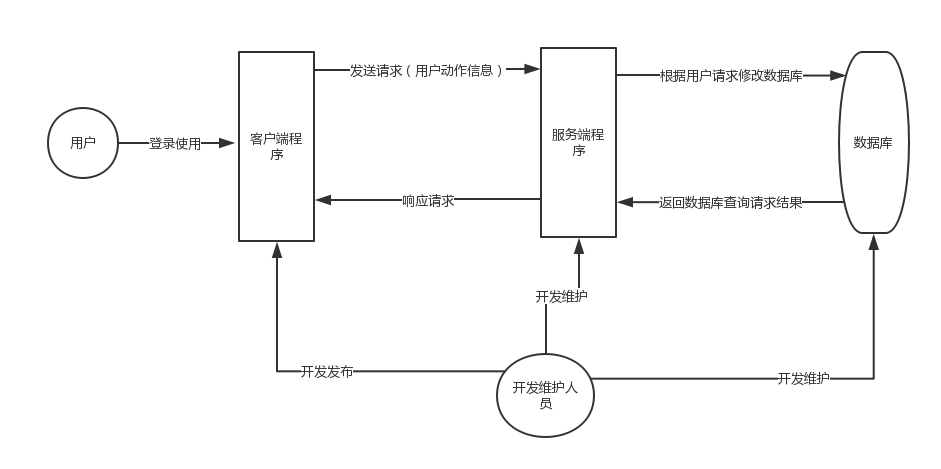
\includegraphics[width=10cm]{zhengti.png}
	\caption{系统基本流程} 
	\label{fig:figure8s}
\end{figure}

\subsection{客户端基本流程}
\begin{figure}[H]
	\centering
	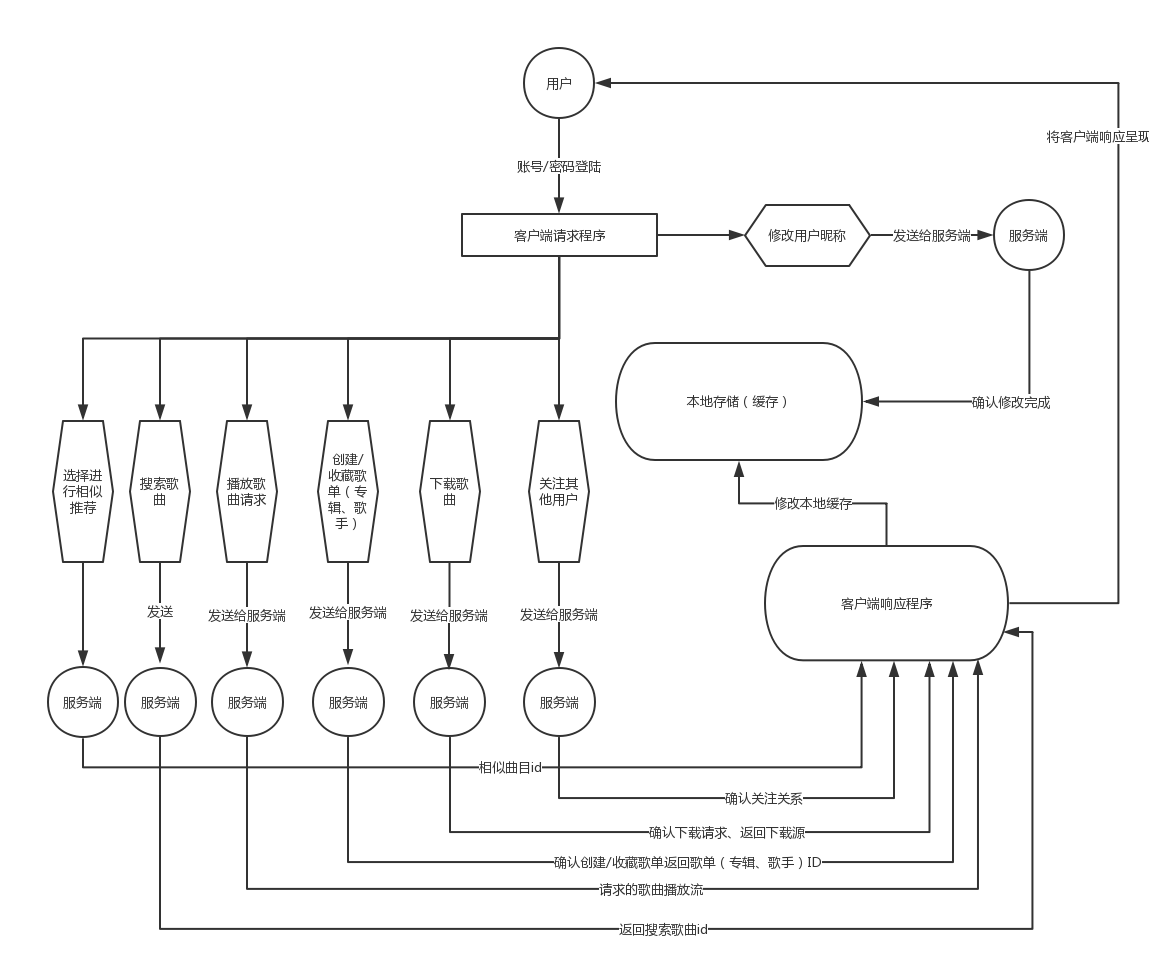
\includegraphics[width=10cm]{kehuduanchuliliucheng.png}
	\caption{客户端基本流程} 
	\label{fig:figure8d}
\end{figure}

在用户移动端上提供一个云平台的客户服务平台,主要目的在于与服务端之间建立通信关

系,产生发送对应的请求与动作,接受服务端的响应。例如接受服务端发送回来的播放的音

频流,调用播放接口对请求的歌曲进行播放,还包括例如缓存功能,缓存最近播放的歌曲在

移动端的存储中,缓存如用户昵称等个人信息。

\subsection{服务器端基本流程}

\begin{figure}[H]
	\centering
	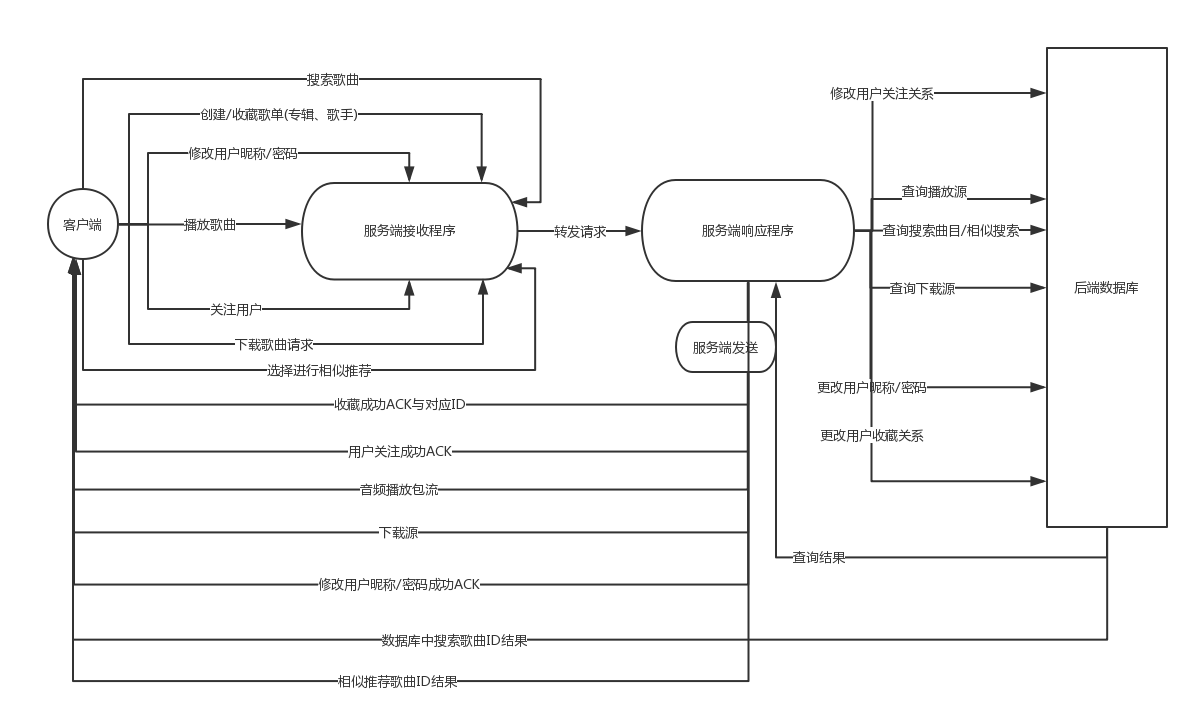
\includegraphics[width=10cm]{fuwuduanchuliliucheng.png}
	\caption{服务器端基本流程} 
	\label{fig:figure8ds}
\end{figure}
接受客户端发送的动作和请求,处理并响应,同时对该请求做出响应,例如前端某用户收藏了某歌单,客户端发送该动作,服务端做出相应的响应,将该歌单来源返回给用户,并修改相应的的数据库信息。当前端发送请求下载某歌曲,服务端响应发送歌曲下载源,对应 播放请求则就是响应发送音频包流。

\subsection{功能1搜索具体流程}

已经登录的用户在搜索栏提交get请求,客户端发送用户搜索请求数据包,提交的内容中包含歌曲的部分关键字,由服务端接收程序验证该请求是否合法,并由服务端处理程序在数据库中进行对应的查询,返回的数据包中包括包含歌曲的ID、歌曲名称、歌曲所属专辑 、歌曲演唱歌手等信息的界面。

\subsection{功能2播放具体流程}

 已经登录的用户在歌曲信息界面发送播放歌曲请求(在线缓存播放),客户端发送的数据包包括歌曲ID号等候选码,由服务端接收程序验证该请求是否合法,服务端处理程序接受请求并在数据库中进行相应搜索,将相应歌曲的音频包流发送回客户端,客户端接收程 序接收音频数据包调用本地接口对该歌曲进行播放。


\subsection{功能3收藏具体流程}


已经登录的用户在歌曲(专辑、歌手)信息界面发送收藏请求(在线缓存播放),客户端发送的数据包包括用户ID和歌曲(专辑、歌手)ID号等候选码,由服务端接收程序验证该请求是否合法,服务端处理程序接受请求并在用户信息数据库中进行相应搜索,修改数据 库中用户收藏关系条目,若成功则返回收藏成功ACK至客户端。

\subsection{功能4下载具体流程}

已经登录的用户在歌曲信息界面发送播放歌曲请求(在线缓存播放),客户端发送的数据包包括歌曲ID号等候选码,由服务端接收程序验证该请求是否合法,服务端处理程序接受请求并在数据库中进行相应搜索,将相应歌曲的下载源客户端,客户端接收程序接收下载源 ,调用本地程序接口,处理下载源请求,将下载源处的歌曲下载至本地存储。

\subsection{功能5关注用户具体流程}

已经登录的用户在其他用户界面发送播放歌曲请求(在线缓存播放),客户端发送的数据包包括发起请求用户的ID和目标用户界面的ID,由服务端接收程序验证该请求是否合法,服务端处理程序接受请求并在数据库中对发起请求用户ID进行相应搜索,将其关注用户中添 加目标用户,并搜索目标用户条目,在其粉丝成员中添加发起请求用户,完成操作后服务端发送关注成功ACK至客户端。

\subsection{功能6相似推荐具体流程}

已经登录的用户在歌曲信息界面发送相似推荐请求,客户端发送的数据包包括所在曲目歌曲ID号等候选码,由服务端接收程序验证该请求是否合法,服务端处理程序接受请求并利用推荐搜索算法在数据库中进行相应搜索,搜索相似曲风的歌曲ID及其他信息并将其发送回 客户端,客户端接收并将歌曲名称进行罗列供用户选择。

\section{功能结构设计}
\subsection{整体结构}
此处应当有一个图和对应的描述。系统如果像微内核那样,划分成核心模块和若干个子系统,此处应当有图示及说明,然后后续几个节应当描述这几个子系统。如果系统像宏内核,那应当说明有哪些紧密联系的模块,并在后续几个节内描述这些模块。
`
\subsection{客户端结构}

\begin{figure}[H]
	\centering
	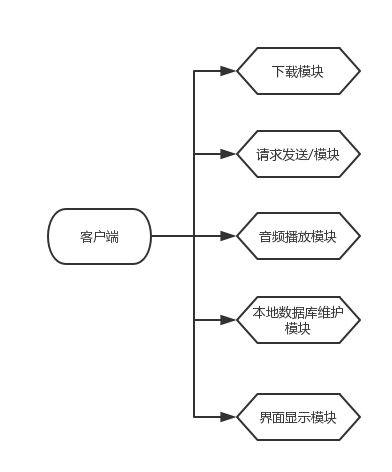
\includegraphics[width=10cm]{kehuduanjiegou.png}
	\caption{客户端结构} 
	\label{fig:figure8asd}
\end{figure}


\subsection{服务器端结构}

\begin{figure}[H]
	\centering
	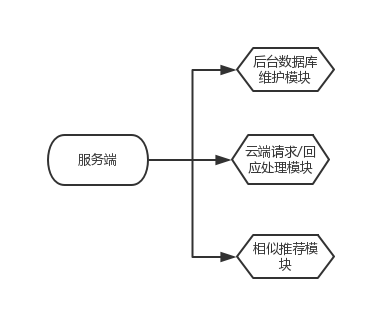
\includegraphics[width=10cm]{fuwuduanjiegou.png}
	\caption{服务器端结构} 
	\label{fig:figure8ass}
\end{figure}




\section{功能需求与程序代码的关系}
[此处指的是不同的需求分配到哪些模块去实现。可按不同的端拆分此表]
\begin{table}[htbp]
\centering
\caption{功能需求与程序代码的关系表} \label{tab:requirement-module}
\begin{tabular}{|c|c|c|c|c|c|c|c|c|c|}
    \hline
    · & 下载模块 & 请求发送/接收模块 & 音频播放模块 & 本地数据库维护模块 & 界面显示模块 & 后台数据库维护模块
     & 云端请求/回应处理模块 & 相似推荐模块 \\
    \hline
    搜索 & · & Y & . & . & .& Y& .& . \\
    \hline
    播放 & · & Y & Y & . & .& Y.& .& . \\
    \hline
    收藏 & · & Y & . & . & .& Y.& Y& . \\
    \hline
    个人信息 & · & Y & . & . & .& Y.& Y& . \\
    \hline
    推荐功能 & · & Y & . & . & .& Y.& Y& Y \\
    \hline
\end{tabular}
\note{各项功能需求的实现与各个程序模块的分配关系}
\end{table}
\chapter{接口设计}
\section{用户接口}
客户端程序是安卓图形交互程序,提供图形化的用户界面

\section{内部接口}
\subsection{下载模块\ 与\ 请求发送/接收模块}
下载模块将下载请求发送给请求发送/接收模块,以进一步处理。请求发送/接收模块在接受到云端送来的数据包后进一步组装成可以被上层模块直接处理的数据。

这两个模块间的通讯是通过操作系统的底层的调用实现的,即两者相互调用并通过操作系统传递消息。

\subsection{下载模块\ 与\ 本地数据库维护模块}
下载模块会将下载的数据保存到本地。这时候本地数据库维护模块会将这个信息保存在本地数据库中。

这两个模块间的通讯是通过操作系统的底层的调用实现的。

\subsection{音频播放模块\ 与\ 本地数据库维护模块}
音频播放模块在要播放本地音乐信息的时候会通过查询本地数据库维护模块,来得到本地保存了哪些音乐文件,以及这些音乐文件的位置。每次通讯的过程是音频播放模块向本地数据库维护模块提出查询请求,本地数据库维护模块处理请求后将结果返回给音频播放模块。

这两个模块间的通讯是通过操作系统的底层的调用实现的。

\subsection{界面显示模块\ 与\ 本地数据库维护模块}
界面显示模块在要显示相关信息的时候会通过查询本地数据库维护模块,来得到本地保存了哪些信息(如用户头像等),以及这些信息文件保存的位置。每次通讯的过程是界面显示模块向本地数据库维护模块提出查询请求,本地数据库维护模块处理请求后将结果返回给界面显示模块。

这两个模块间的通讯是通过操作系统的底层的调用实现的。

\subsection{音频播放模块\ 与\ 请求发送/接收模块}
当要播放网络中的歌曲时,音频播放模块首先向请求发送/接收模块发送播放网络流媒体的请求。当服务器发送的流媒体数据到达本机之后,先通过请求发送/接收模块将数据封装为可以被上层软件直接使用的数据,然后再将这个数据发送给音频播放模块。

这两个模块间的通讯是通过操作系统的底层的调用实现的。

\subsection{请求发送/接收模块\ 与\ 云端请求/回应处理模块}
请求发送/接收模块和云端请求。回应处理模块是手机客户端与云端服务器之间进行通讯的唯一方式。请求发送/接收模块处理客户端中所用访问云端数据的请求,将这些请求封装为数据包,以IP报文的格式发送出去。而云端请求/回应处理模块会在接收到这些IP报文后将这些报文解析为上层可用的数据以进一步使用。在云端数据准备好后,云端请求/回应处理模块将这些云端的数据封装为数据包,以IP报文的格式发送给客户端。而客户端在接收到这些数据后,将这些数据解析为客户端上层软件可以直接使用的数据,在发送给相应的上层模块。

这两个模块中的通讯通过网络实现,将借助TCP/IP协议进行通讯。

\subsection{后台数据库维护模块\ 与\ 云端请求/回应处理模块}
当云端接收到访问后台数据库的请求时,它会在将这个请求解析出来后,将请求转发给后台数据库维护模块。后台数据库接收到云端请求/回应处理模块后将数据从后台数据库中查询出来。待数据处理准备好之后,数据被发送给云端请求/回应模块。

这两个模块之间的通讯通过云端服务器中的操作系统的调用和信息传递机制完成。

\subsection{后台数据库维护模块\ 与\ 相似推荐模块}
相似推荐模块要计算和查找相似的推荐时,会向后台数据维护模块发出访问一些后台数据库中数据的请求。后代数据库维护模块接收到这些请求后会将数据准备好,然后发送给相似推荐模块进行进一步的计算和分析。

这两个模块之间的通讯通过云端服务器中的操作系统的调用和信息传递机制完成。

\subsection{云端请求/回应处理模块\ 与\ 相似推荐模块}
到达云端的请求还有可能是对相似推荐的请求。这时候,云端请求/回应模块将这个请求发送给相似推荐模块。相似推荐模块会进行计算后得到一些相似的歌曲信息。这些信息会由相似推荐模块发送给云端请求/回应处理模块。

这两个模块之间的通讯通过云端服务器中的操作系统的调用和信息传递机制完成。


\chapter{数据结构设计}
\section{逻辑结构设计}
\subsection{用户管理系统数据结构设计}
讲述本系统内需要什么数据结构。这指的是程序运行过程中维护的数据结构。只是举个例子,此处应和3.3一致。
\subsection{客户端数据结构}

1.下载模块:

维护数据结构:下载源字符串类型,缓冲区,通信计时

客户端的下载模块需要维护一个字符串类型来存储服务端返回的下载源,下载模块调用本地接口请求目标源的数据包,下载模块并需要动态缓冲区类型来从下载源存储正在下载的数据,数据结构通信计时器查看是否发生请求超时或者丢包等情况影响下载。



2.请求发送/接收模块:

请求接收模块是一个基本的重要模块,它需要维护数据结构有: 请求/接收包数据规模,数据缓冲区,通信计时,校验串

请求、接收模块是对数据请求和响应的发送与处理模块,数据缓冲区用来存储数据包的内容,通信计时器和校验串为了保证通信的正常进行和数据包的完整性,动态变化的请求/接收数据规模数据结构设定为为数据缓冲区分配存储空间的大小。

3.音频播放模块(包括流媒体):

维护的数据结构: 音频数据缓冲区,进度参数,计时器

根据云端发回的音频数据,客户端需要将音频数据载入音频数据缓冲区,进度参数为播放该歌曲的进度,可由前端用户更改跳转至对应的音频数据缓冲区位置,计时器为该歌曲所播放的时间随播放进行动态变化。



4.本地数据库维护模块:

维护数据结构:用户ID和权限,与云端同步的标志位信息,数据库操作类型

根据当前登录的用户ID和其拥有的权限可拥有对本地数据的一定访问权限,根据与云端同步的标志位信息判断该维护动作是否合法,并利用数据库操作类型选定需要进行的数据库动作。

5.界面显示模块:
维护数据结构:界面结构信息、各结构块规模和结构体内容

根据设定的各界面结构信息,各结构体块规模,配合结构体内容向用户展示对应的界面窗口。

\subsection{服务端数据结构}

后端数据库维护模块:

数据结构:

数据库操作:
\begin{itemize}
	\item 操作表对象;
	\item 操作类型
	\item 操作值
	\item 操作语句
	\item 发生时间
	\item 是否成功
\end{itemize}




表对象信息:
\begin{itemize}
	\item 表名
	\item 表记录数
	\item 表最后一次操作
	\item 表可用性
\end{itemize}


云端请求/回应:
\begin{itemize}
	\item 请求来源
	\item 目标URL
	\item 请求类型
	\item 请求资源
	\item 请求源代码
	\item 发生时间
	\item 是否已回应
\end{itemize}



回应:{
\begin{itemize}
	\item 回应目标URL
	\item 回应来源
	\item 回应信息体
	\item 回应对应请求
	\item 回应时间
	\item 是否已送达
\end{itemize}


相似推荐模块:
\begin{itemize}
	\item 歌曲id
	\item 歌曲名称
	\item 歌曲标签
\end{itemize}



\section{物理结构设计}
无

\chapter{数据库设计}
\section{数据库环境说明}
本系统的数据库采用MySQL数据库系统

\section{数据库的命名规则}

名称的命名方式选用头字母大写(头分法)

不允许单词缩写,基本采用含义连拼的方式

表名是复数,大写

字段带上类型前缀(有利于数据库维护时对数据库进行操作与维护),中间用下划线分割:

EXP:

string——s

integer——i

long——l

char——c

double——lf

float——f

\section{逻辑设计}
\begin{figure}[H]
	\centering
	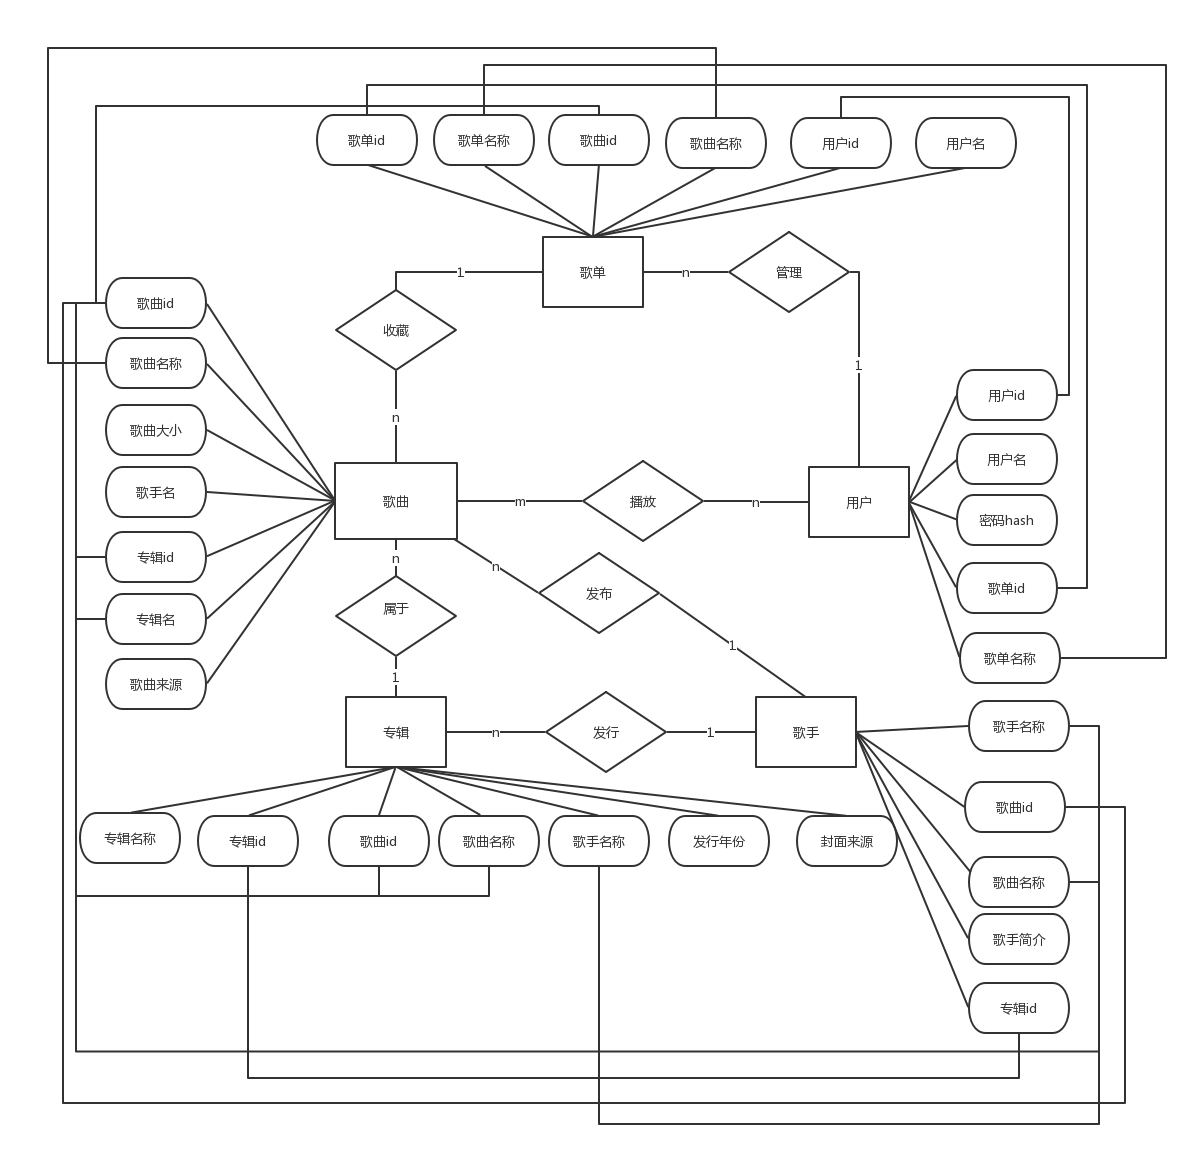
\includegraphics[width=10cm]{ER.png}
	\caption{逻辑设计图} 
	\label{fig:figure8er}
\end{figure}


\section{物理设计}
\subsection{数据库产品}
瑞典MySQL AB 公司的MySQL数据库,非分布式

\subsection{实体属性、类型、精度}



\subsubsection{歌曲数据表设计}
\begin{table}[htbp]
	\centering
	\caption{歌曲数据表Songs设计} \label{tab:songs-database}
	\begin{tabular}{|c|c|c|c|c|}
		\hline
		字段名 & 类型 & 大小 & 说明 & 备注 \\
		\hline
		s\_id & char & 64 & 歌曲的唯一标识符 & 主键\\
		\hline
		s\_name & char & 128 & 歌曲的名称 &  \\
		\hline
		f\_size & float & 1 & 歌曲文件的大小 & \\
		\hline
		s\_artist\_name & char & 64 & 歌手的名称 & 外键,来自Artists表 \\
		\hline
		s\_album\_id & char & 64 & 歌曲所属专辑的id & 外键,来自Albums表 \\
		\hline
		s\_album\_name & char & 128 & 歌曲所属专辑的名称 & \\
		\hline
		s\_source & char & 512 & 歌曲文件的来源,URL & \\
		\hline
	\end{tabular}
	\note{歌曲数据表Songs设计}
\end{table}

\subsubsection{专辑数据表设计}
\begin{table}[htbp]
	\centering
	\caption{专辑数据表Albums设计} \label{tab:albums-database}
	\begin{tabular}{|c|c|c|c|c|}
		\hline
		字段名 & 类型 & 大小 & 说明 & 备注 \\
		\hline
		s\_id & char & 64 & 专辑的唯一标识符 & 主键 \\
		\hline
		s\_song\_id & char & 64 & 专辑内某一歌曲的唯一标识符 & 外键,来自Songs表 \\
		\hline
		s\_song\_name & char & 128 & 专辑内某一歌曲的名称 & \\
		\hline
		s\_artist\_name & char & 64 & 专辑所属歌手的唯一标识符 & 外键,来自Artists表 \\
		\hline
		s\_publi\_date & date & 1 & 专辑发行日期 & \\
		\hline
		s\_cover\_src & char & 512 & 专辑封面的来源URL & \\
		\hline
	\end{tabular}
	\note{专辑数据表Albums设计}
\end{table}

\subsubsection{歌手数据表设计}
\begin{table}[htbp]
	\centering
	\caption{歌手数据表Artists设计} \label{tab:artists-database}
	\begin{tabular}{|c|c|c|c|c|}
		\hline
		字段名 & 类型 & 大小 & 说明 & 备注 \\
		\hline
		s\_name & char & 64 & 歌手的唯一标识符,也是歌手的名字 & 主键 \\
		\hline
		s\_song\_id & char & 64 & 歌手所发布歌曲的id & 外键,来自Songs表 \\
		\hline
		s\_song\_name & char & 128 & 歌手所发布歌曲的名称 & \\
		\hline
		s\_intro & char & 1024 & 歌手的简介信息 & \\
		\hline
	\end{tabular}
	\note{歌手数据表Artists设计}
\end{table}

\subsubsection{歌单数据表设计}
\begin{table}[htbp]
	\centering
	\caption{歌单数据表Lists设计} \label{tab:lists-database}
	\begin{tabular}{|c|c|c|c|c|}
		\hline
		字段名 & 类型 & 大小 & 说明 & 备注 \\
		\hline
		s\_id & char & 64 & 歌单的唯一标识符 & 主键 \\
		\hline
		s\_name & char & 128 & 歌单的名称 & \\
		\hline
		s\_song\_id & char & 64 & 歌单内某首歌曲的id & 外键,来自Songs表 \\
		\hline
		s\_song\_name & char & 128 & 歌单内某首歌曲的名称 & \\
		\hline
		s\_user\_id & char & 64 & 歌单所属用户的id & 外键,来自Users表\\
		\hline
		s\_user\_name & char & 128 & 歌单所属用户的用户名 & \\
		\hline
	\end{tabular}
	\note{歌单数据表Lists设计}
\end{table}

\subsubsection{用户数据表设计}
\begin{table}[htbp]
	\centering
	\caption{用户数据表Users设计} \label{tab:users-database}
	\begin{tabular}{|c|c|c|c|c|}
		\hline
		字段名 & 类型 & 大小 & 说明 & 备注 \\
		\hline
		s\_id & char & 64 & 用户的唯一标识符 & 主键 \\
		\hline
		s\_name & char & 128 & 用户名 & \\
		\hline
		s\_passwd & char & 512 & 用户密码的hash值 & \\
		\hline
		s\_list\_id & char & 64 & 用户的歌单的id & 外键,来自Lists表 \\
		\hline
		s\_list\_name & char & 128 & 用户歌单的名称 & \\
		\hline
	\end{tabular}
	\note{用户数据表Users设计}
\end{table}

\section{安全性设计}
备份和容灾设计。

设置一份与生产环境一致的容灾节点,利用磁盘介质在容灾节点保留一份生产系统每天的原始数据

在应用层面上,本地节点使用Cluster Server实现主机高可用性,防止主机故障.

在数据层面山,在本地先形成一套主机系统和业务数据的磁盘备份,并每隔8小时在后台将本地备份数据复制到远程容灾节点(周期复制),异地节点恢复主节点数据,以实现主备节点的数据同步。 

主节点和灾备节点在硬盘上至少保持6个月内的系统历史数据。 

\section{数据库管理与维护说明}
对于数据库的维护,随时对数据库中的信息加以调试和保存备份。同样需要个工作人员进行系统的分析和用户的反馈,对系统进行升级以及功能的完善。同时保证系统安全有序的运行。
\chapter{界面设计}
\section{客户端界面}
\vspace{3ex}
\begin{figure}[H]
	\centering
	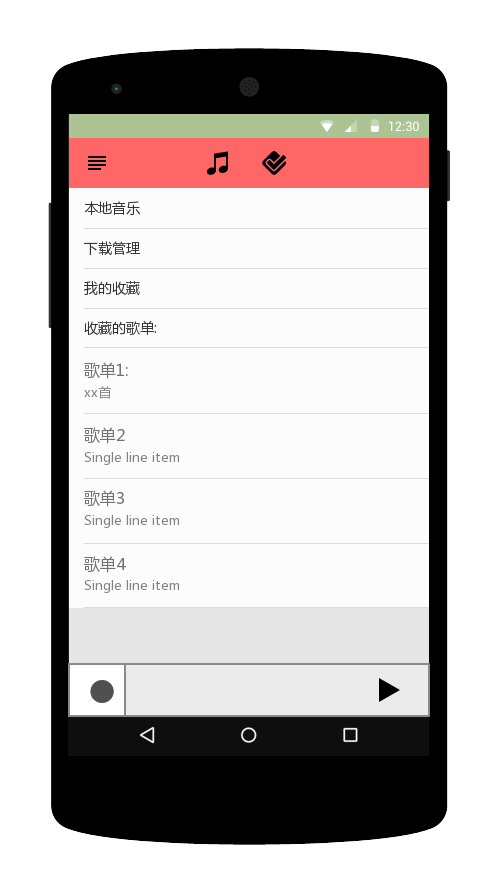
\includegraphics[width=10cm]{kehuduan.png}
	\caption{客户端界面} 
	\label{fig:figure8}
\end{figure}


这里是用户打开应用程序时的界面,界面分为两部分:主页面和播放栏.


播放栏在大部分情况下都会存在,是一个长久存在的ui组件,用于对播放状态进行控制,用户可以点击播放按钮,控制当前按钮的播放.或者通过点击位于播放栏左侧的图标,进入歌曲详情界面.对于歌曲详情界面,下面会进行展示


主页面是一个包含两项的ViewPager,其中第一个页面(左边的页面)是我的音乐界面栏.用户可以通过点击相应选型进入其他界面:
\begin{itemize}
	\item 最近播放:进入最近播放界面
	\item 下载管理:进入下载管理界面
	\item 我的收藏:进入我的收藏界面
	\item 歌单X:进入歌单界面
\end{itemize}

用户可以点击标题栏右边的按钮进入动态主页界面.

用户可以通过点击标题栏最左侧的列表按钮,或者从左向右进行拖拽打开用户选项栏


\section{登录界面}
\begin{figure}[H]
	\centering
	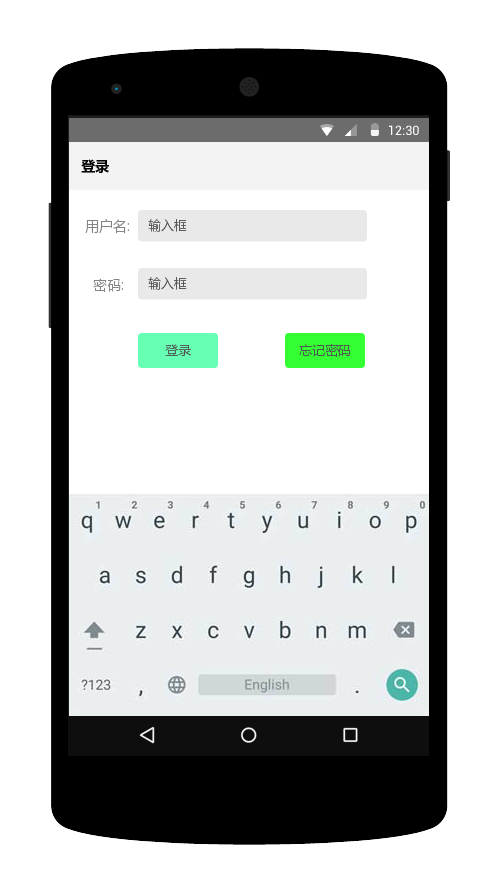
\includegraphics[width=10cm]{denglu.png}
	\caption{登录界面} 
	\label{fig:figure1ss8}
\end{figure}

在用户登录界面,用户在输入框中输入用户名及密码,点击登录按钮后即可完成登陆操作.如果登录成功,返回客户端界面,否则,留在登录界面,显示错误信息.如果用户点击忘记密码按钮,则调用系统的WebView访问预设的密码更改页面.

\section{播放界面}

\begin{figure}[H]
	\centering
	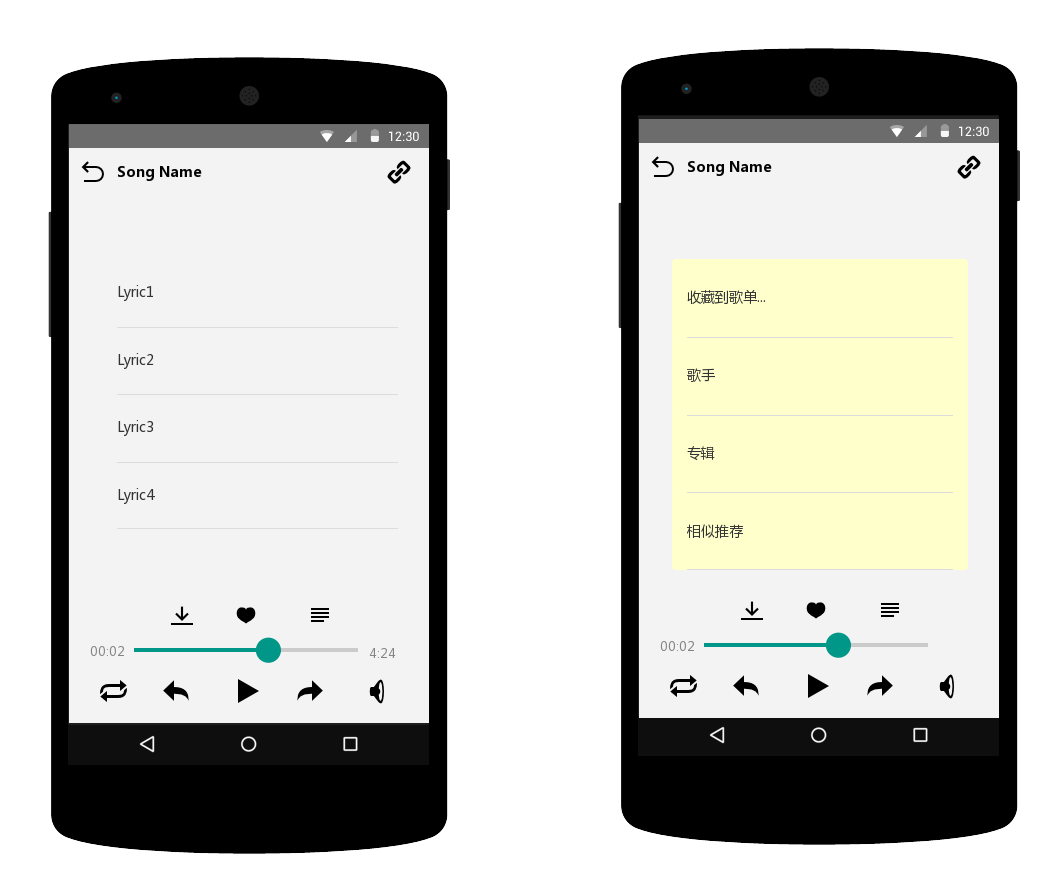
\includegraphics[width=10cm]{bofang.png}
	\caption{播放界面} 
	\label{fig:figure1s8}
\end{figure}

用户通过点击歌曲项进入播放界面时,将进入左图所示的歌曲界面.用户通过点击界面上的按钮将进行不同操作
\begin{itemize}
	\item 标题栏左边的返回按钮:将返回上一个活动
	\item 标题栏右边的链接按钮:进行分享操作,其行为由系统定义
	\item 底层
\end{itemize}	



底层栏:
\begin{itemize}
	\item 最左侧循环按钮:切换播放方式,包括列表循环等
	\item 上一首:播放上一首歌曲
	\item 播放/暂停:进行歌曲的播放/暂停,图标相应发生变化
	\item 下一首:播放下一首歌曲
	\item 喇叭:设置播放音量
\end{itemize}


进度条:
\begin{itemize}
	\item 进度条:用户通过拖动进度条控制播放进度
\end{itemize}



进度条上方栏:
\begin{itemize}
	\item 下载按钮:下载当前歌曲
	\item 收藏按钮:将当前歌曲加入/删除到"我最喜爱的歌曲"歌单中
	\item 选项按钮:展开选项栏,效果如右图所示
\end{itemize}



展开的选项栏:
\begin{itemize}
	\item 收藏到歌单:收藏到选定的用户歌单中
	\item 歌手:打开该歌手界面
	\item 专辑:打开该专辑界面
	\item 相似推荐:打开相似推荐界面
\end{itemize}


\section{专辑界面}

\begin{figure}[H]
	\centering
	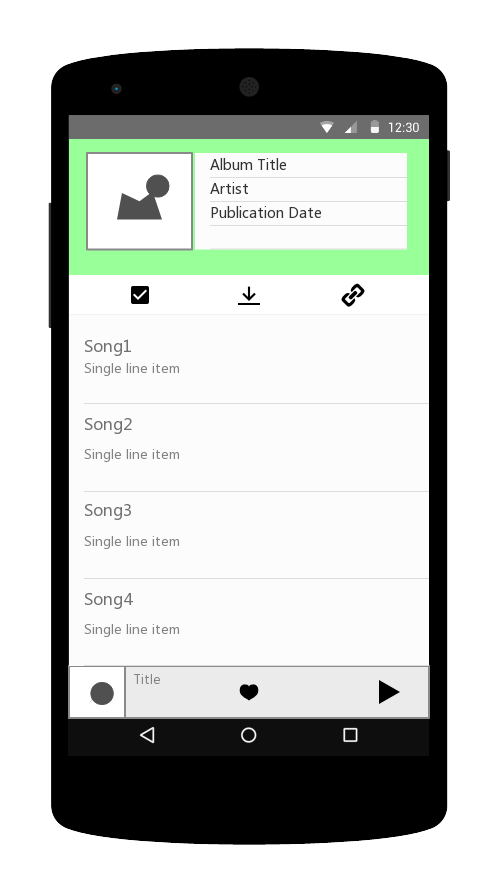
\includegraphics[width=10cm]{zhuanji.png}
	\caption{专辑界面} 
	\label{fig:figure118}
\end{figure}

专辑界面显示了一个专辑的基本信息,包括专辑封面,专辑名称,歌手,发行日期等信息,同时,以歌曲项列表的形式显示专辑内的所有歌曲.
底部播放栏前面已经介绍,不再赘述.

\begin{itemize}
	\item 选择按钮:用户点击后可以选择将专辑内所有歌曲加入指定歌单中
	\item 下载按钮:用户点击后可以下载专辑内所有歌曲
	\item 分享按钮:用户点击后可以将专辑分享给其他应用,行为由系统确定.
\end{itemize}

\section{歌单界面}
歌单界面显示了一个歌单的基本信息,其界面和专辑界面类似,但是没有歌手,发行日期信息,其他行为表现和专辑界面完全一致,不再赘述.

\section{歌手界面}
\begin{figure}[H]
	\centering
	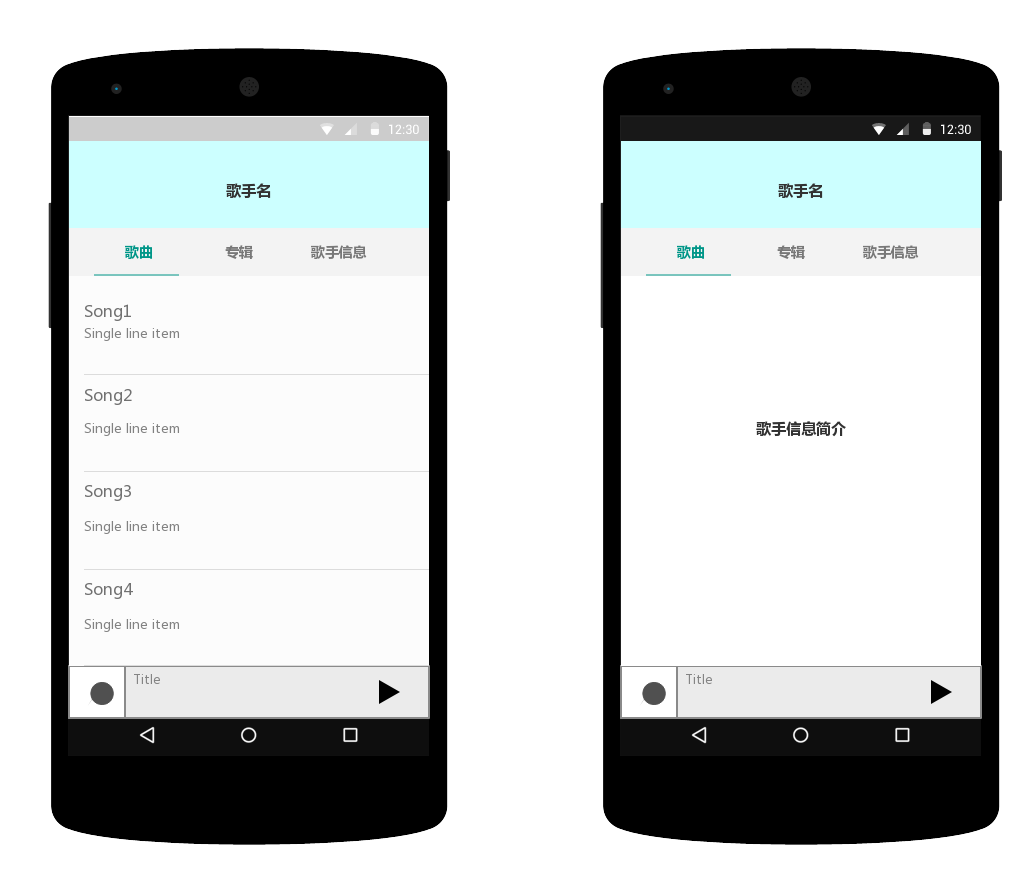
\includegraphics[width=10cm]{geshou.png}
	\caption{歌手界面} 
	\label{fig:figure1v8}
\end{figure}

用户可以在三个选项卡内进行选择,可以找到该名歌手的所有歌曲,所有专辑和歌手简介三个页面.

\begin{itemize}
	\item 所有歌曲界面:用户通过点击某一歌曲项,可以进入该歌曲的歌曲界面
	\item 所有专辑界面:用户通过点击某一专辑项,可以进入该专辑的专辑界面
	\item 歌手简介界面:只显示简介文本
\end{itemize}


\chapter{出错处理设计}
\section{数据库出错处理}
当保存用户信息的数据库出错时,暂停整个用户系统的服务,涉及到用户信息的所有操作向客户端返回报错响应.

当歌曲数据库发生错误时,暂停整个系统的服务,对用户发送的所有搜索,播放,下载请求返回报错响应.

当专辑,歌手数据库发生错误时,对于一切进入专辑/歌手界面的操作返回报错相应.

当歌单数据库发生错误时,对于一切更新云端歌单数据库的请求返回报错相应,此时客户端应使用本地维护的歌单数据库.

在数据库发生错误时,首先尝试使用日志恢复到正常状态;如果不行,尝试恢复本地保存的备份数据;如果本地备份数据也已损坏,尝试恢复容灾节点的备份数据.如果以上操作均失败,则云端自行恢复数据库已变的不可能,向客户发出服务已失效的公告.对于歌单数据库发生的错误,考虑以下解决方案:
在已经告知用户云端数据库已毁坏的情况下,由客户端向云端发送保存在本地的歌单数据,以最大程度的恢复数据.

\section{某模块失效处理}

是否整个系统暂停服务,还是维持最小服务状态、如何尽快恢复服务还是删库跑路等。
\subsection{本地模块失效处理}

\subsubsection{下载模块}

当下载模块失效时,暂停下载模块的工作,请求模块不再发送下载请求,当确定模块失效是广泛存在时,由开发者对bug进行修复,并尽快推送更新给所有用户.

\subsubsection{音频播放模块}

当音频播放模块失效时,暂停所有播放功能,其他模块正常工作,当确定模块失效是广泛存在时,由开发者对bug进行修复,并尽快推送更新给所有用户.

\subsubsection{请求发送/接收模块}

当请求发送/接收模块失效时,暂停下载模块的工作,其他模块正常工作,首先由本地确定失效原因,如果确定失效原因由代码内部的错误引起,则不断尝试向云端发送错误信息.当确定模块失效是广泛存在时,由开发者对bug进行修复,并尽快推送更新给所有用户.

\subsubsection{本地数据库维护模块}

当本地数据库维护模块失效时,暂停所有模块的工作,尝试清空本地数据库.如果清空数据库后本地数据库维护仍处于失效状态,则认定该应用已不可用,向用户发出错误信息,向用户建议重新安装应用程序.当确定模块失效是广泛存在时,由开发者对bug进行修复,并尽快推送更新给所有用户.

\subsubsection{界面显示模块}

当界面显示模块失效时,暂停所有模块的工作,认定该应用已不可用,向用户建议重新安装应用程序.当确定模块失效是广泛存在时,由开发者对bug进行修复,并尽快推送更新给所有用户.

\subsection{云端模块失效处理}

\subsubsection{后台数据库维护模块}

当后台数据库维护模块失效时,实行上一节介绍的数据库出错处理操作,恢复数据库数据.如果后台数据库维护模块的失效不是由数据错误引起的,则尽快对代码bug进行修复.

后台数据库维护模块失效时,一切发往云端的请求都将收到一个保存响应,同时暂停云端上其他模块的工作.

\subsubsection{云端请求/回应处理模块}

当云端请求/回应处理模块失效时,暂停相似推荐模块的工作,尽快对代码bug进行修复.

\subsubsection{相似推荐模块}

当相似推荐模块失效时,在云端请求/回应处理模块对所有相似推荐的请求返回报错相应,尽快对代码bug进行修复.

\chapter{安全保密设计}
可能的内容包括保密性、是否采取加密传输、密钥如何分发和管理等。

\subsection{保密性}

对设计用户信息的传输进行保密,包括:
\begin{itemize}
	\item 用户登录
	\item 用户注销
	\item 收藏操作
	\item 密码修改
\end{itemize}

\subsection{加密传输}

对于除 流媒体传输和下载 外所有本地与云端的数据交换,采用https进行传输.
\chapter{维护设计}
可能的内容包括数据库的日常备份、压缩、维护等。

\subsection{备份}

对以下数据库进行完全备份:
\begin{itemize}
	\item Songs
	\item Artists
	\item Albums
	\item Users
	\item Lists
\end{itemize}

对于数据库备份的操作,在6.6节中已经介绍,不再赘述.

同时,对收到的以下请求和结果进行备份:
\begin{itemize}
	\item 收藏操作
	\item 歌单创建操作
	\item 用户信息更改操作
\end{itemize}

\subsection{维护}

每天2:00进行以下项目的检验:
\begin{itemize}
	\item 云端网络的可达性
	\item 流媒体连接的速度
	\item 数据库内容的正确性(检验和)
\end{itemize}


%\chapter{图片}
本章展示图片相关用法。

\section{示例}
\begin{figure}[ht]
\centering

\includegraphics[width=10cm]{ustc_logo_fig}
\caption{测试图片} \label{fig:figure1}
\end{figure}

\section{带图注的图}
\begin{figure}[ht]
\centering

\includegraphics[width=10cm]{ustc_logo_fig}
\caption{带图注的图片}\label{fig:noted-figure}
\note{the solid lines represent the time histogram of the spontaneous activities of an old monkey cell(gray) and a young monkey cell (black). The bin-width is 1}
\end{figure}

%\chapter{表格}

\section{A Simple Table}
\begin{table}[htbp]
\centering
\caption{这里是表的标题} \label{tab:simpletable}
\begin{tabular}{|c|c|}
    \hline
    a & b \\
    \hline
    c & d \\
    \hline
\end{tabular}
\note{这里是表的注释}
\end{table}

\section{长表格}
\begin{longtable}{ccc}
% 首页表头
\caption[长表格演示]{长表格演示} \label{tab:longtable} \\
\toprule[1.5pt]
名称  & 说明 & 备注\\
\midrule[1pt]
\endfirsthead
% 续页表头
\caption[]{长表格演示(续)} \\
\toprule[1.5pt]
名称  & 说明 & 备注 \\
\midrule[1pt]
\endhead
% 首页表尾
\hline
\multicolumn{3}{r}{\small 续下页}
\endfoot
% 续页表尾
\bottomrule[1.5pt]
\endlastfoot

AAAAAAAAAAAA   &   BBBBBBBBBBB   &   CCCCCCCCCCCCCC   \\
AAAAAAAAAAAA   &   BBBBBBBBBBB   &   CCCCCCCCCCCCCC   \\
AAAAAAAAAAAA   &   BBBBBBBBBBB   &   CCCCCCCCCCCCCC   \\
AAAAAAAAAAAA   &   BBBBBBBBBBB   &   CCCCCCCCCCCCCC   \\
AAAAAAAAAAAA   &   BBBBBBBBBBB   &   CCCCCCCCCCCCCC   \\
AAAAAAAAAAAA   &   BBBBBBBBBBB   &   CCCCCCCCCCCCCC   \\
AAAAAAAAAAAA   &   BBBBBBBBBBB   &   CCCCCCCCCCCCCC   \\
AAAAAAAAAAAA   &   BBBBBBBBBBB   &   CCCCCCCCCCCCCC   \\
AAAAAAAAAAAA   &   BBBBBBBBBBB   &   CCCCCCCCCCCCCC   \\
AAAAAAAAAAAA   &   BBBBBBBBBBB   &   CCCCCCCCCCCCCC   \\
AAAAAAAAAAAA   &   BBBBBBBBBBB   &   CCCCCCCCCCCCCC   \\
AAAAAAAAAAAA   &   BBBBBBBBBBB   &   CCCCCCCCCCCCCC   \\
AAAAAAAAAAAA   &   BBBBBBBBBBB   &   CCCCCCCCCCCCCC   \\
AAAAAAAAAAAA   &   BBBBBBBBBBB   &   CCCCCCCCCCCCCC   \\
AAAAAAAAAAAA   &   BBBBBBBBBBB   &   CCCCCCCCCCCCCC   \\
AAAAAAAAAAAA   &   BBBBBBBBBBB   &   CCCCCCCCCCCCCC   \\
AAAAAAAAAAAA   &   BBBBBBBBBBB   &   CCCCCCCCCCCCCC   \\
AAAAAAAAAAAA   &   BBBBBBBBBBB   &   CCCCCCCCCCCCCC   \\
AAAAAAAAAAAA   &   BBBBBBBBBBB   &   CCCCCCCCCCCCCC   \\
AAAAAAAAAAAA   &   BBBBBBBBBBB   &   CCCCCCCCCCCCCC   \\
AAAAAAAAAAAA   &   BBBBBBBBBBB   &   CCCCCCCCCCCCCC   \\
AAAAAAAAAAAA   &   BBBBBBBBBBB   &   CCCCCCCCCCCCCC   \\
AAAAAAAAAAAA   &   BBBBBBBBBBB   &   CCCCCCCCCCCCCC   \\
AAAAAAAAAAAA   &   BBBBBBBBBBB   &   CCCCCCCCCCCCCC   \\
AAAAAAAAAAAA   &   BBBBBBBBBBB   &   CCCCCCCCCCCCCC   \\
AAAAAAAAAAAA   &   BBBBBBBBBBB   &   CCCCCCCCCCCCCC   \\
AAAAAAAAAAAA   &   BBBBBBBBBBB   &   CCCCCCCCCCCCCC   \\
AAAAAAAAAAAA   &   BBBBBBBBBBB   &   CCCCCCCCCCCCCC   \\
AAAAAAAAAAAA   &   BBBBBBBBBBB   &   CCCCCCCCCCCCCC   \\
AAAAAAAAAAAA   &   BBBBBBBBBBB   &   CCCCCCCCCCCCCC   \\
AAAAAAAAAAAA   &   BBBBBBBBBBB   &   CCCCCCCCCCCCCC   \\
AAAAAAAAAAAA   &   BBBBBBBBBBB   &   CCCCCCCCCCCCCC   \\
AAAAAAAAAAAA   &   BBBBBBBBBBB   &   CCCCCCCCCCCCCC   \\
AAAAAAAAAAAA   &   BBBBBBBBBBB   &   CCCCCCCCCCCCCC   \\
AAAAAAAAAAAA   &   BBBBBBBBBBB   &   CCCCCCCCCCCCCC   \\
AAAAAAAAAAAA   &   BBBBBBBBBBB   &   CCCCCCCCCCCCCC   \\
\end{longtable}

%\chapter{算法环境}
模板中使用 \texttt{algorithm2e} 宏包实现算法环境。关于该宏包的具体用法,
请阅读宏包的官方文档。

\begin{algorithm}[htbp]
\SetAlgoLined
\KwData{this text}
\KwResult{how to write algorithm with \LaTeX2e }

initialization\;
\While{not at end of this document}{
    read current\;
    \eIf{understand}{
        go to next section\;
        current section becomes this one\;
    }{
        go back to the beginning of current section\;
    }
}
\caption{算法示例1}
\label{algo:algorithm1}
\end{algorithm}

\IncMargin{1em}
\begin{algorithm}
\SetKwData{Left}{left}\SetKwData{This}{this}\SetKwData{Up}{up}
\SetKwFunction{Union}{Union}\SetKwFunction{FindCompress}{FindCompress}
\SetKwInOut{Input}{input}\SetKwInOut{Output}{output}

\Input{A bitmap $Im$ of size $w\times l$}
\Output{A partition of the bitmap}
\BlankLine
\emph{special treatment of the first line}\;
\For{$i\leftarrow 2$ \KwTo $l$}{
    \emph{special treatment of the first element of line $i$}\;
    \For{$j\leftarrow 2$ \KwTo $w$}{\label{forins}
        \Left$\leftarrow$ \FindCompress{$Im[i,j-1]$}\;
        \Up$\leftarrow$ \FindCompress{$Im[i-1,]$}\;
        \This$\leftarrow$ \FindCompress{$Im[i,j]$}\;
        \If(\tcp*[h]{O(\Left,\This)==1}){\Left compatible with \This}{\label{lt}
            \lIf{\Left $<$ \This}{\Union{\Left,\This}}
            \lElse{\Union{\This,\Left}}
        }
        \If(\tcp*[f]{O(\Up,\This)==1}){\Up compatible with \This}{\label{ut}
        \lIf{\Up $<$ \This}{\Union{\Up,\This}}
        \tcp{\This is put under \Up to keep tree as flat as possible}\label{cmt}
        \lElse{\Union{\This,\Up}}\tcp*[h]{\This linked to \Up}\label{lelse}
        }
    }
    \lForEach{element $e$ of the line $i$}{\FindCompress{p}}
}
\caption{算法示例2}\label{algo_disjdecomp}
\label{alog:algorithm2}
\end{algorithm}\DecMargin{1em}

%\chapter{代码环境}
模板中使用 \texttt{listings} 宏包实现代码环境。详细用法见宏包的官方说明文档。

以下是代码示例,可以在文中任意位置引用\autoref{first-code} 。
\begin{lstlisting}[language=C, caption=示例代码, label={code:first-code}]
#include <stdio.h>

int main( )
{
    printf("hello, world\n");
    return 0;
}
\end{lstlisting}

%\chapter{引用文献标注}

\section{著者-出版年制标注法}

\noindent
\verb|\citestyle{ustcauthoryear}|
\citestyle{ustcauthoryear}

\noindent
\begin{tabular}{l@{\quad$\Rightarrow$\quad}l}
  \verb|\cite{knuth86a}| & \cite{knuth86a}\\
  \verb|\citet{knuth86a}| & \citet{knuth86a}\\
  \verb|\citet[chap.~2]{knuth86a}| & \citet[chap.~2]{knuth86a}\\[0.5ex]
  \verb|\citep{knuth86a}| & \citep{knuth86a}\\
  \verb|\citep[chap.~2]{knuth86a}| & \citep[chap.~2]{knuth86a}\\
  \verb|\citep[see][]{knuth86a}| & \citep[see][]{knuth86a}\\
  \verb|\citep[see][chap.~2]{knuth86a}| & \citep[see][chap.~2]{knuth86a}\\[0.5ex]
  \verb|\citet*{knuth86a}| & \citet*{knuth86a}\\
  \verb|\citep*{knuth86a}| & \citep*{knuth86a}\\
\end{tabular}

\noindent
\begin{tabular}{l@{\quad$\Rightarrow$\quad}l}
  \verb|\citet{knuth86a,tlc2}| & \citet{knuth86a,tlc2}\\
  \verb|\citep{knuth86a,tlc2}| & \citep{knuth86a,tlc2}\\
  \verb|\cite{knuth86a,knuth84}| & \cite{knuth86a,knuth84}\\
  \verb|\citet{knuth86a,knuth84}| & \citet{knuth86a,knuth84}\\
  \verb|\citep{knuth86a,knuth84}| & \citep{knuth86a,knuth84}\\
\end{tabular}

\section{顺序编码制标注法}

\noindent
\verb|\citestyle{ustcnumerical}|
\citestyle{ustcnumerical}

\noindent
\begin{tabular}{l@{\quad$\Rightarrow$\quad}l}
  \verb|\cite{knuth86a}| & \cite{knuth86a}\\
  \verb|\citet{knuth86a}| & \citet{knuth86a}\\
  \verb|\citet[chap.~2]{knuth86a}| & \citet[chap.~2]{knuth86a}\\[0.5ex]
  \verb|\citep{knuth86a}| & \citep{knuth86a}\\
  \verb|\citep[chap.~2]{knuth86a}| & \citep[chap.~2]{knuth86a}\\
  \verb|\citep[see][]{knuth86a}| & \citep[see][]{knuth86a}\\
  \verb|\citep[see][chap.~2]{knuth86a}| & \citep[see][chap.~2]{knuth86a}\\[0.5ex]
  \verb|\citet*{knuth86a}| & \citet*{knuth86a}\\
  \verb|\citep*{knuth86a}| & \citep*{knuth86a}\\
\end{tabular}

\noindent
\begin{tabular}{l@{\quad$\Rightarrow$\quad}l}
  \verb|\citet{knuth86a,tlc2}| & \citet{knuth86a,tlc2}\\
  \verb|\citep{knuth86a,tlc2}| & \citep{knuth86a,tlc2}\\
  \verb|\cite{knuth86a,knuth84}| & \cite{knuth86a,knuth84}\\
  \verb|\citet{knuth86a,knuth84}| & \citet{knuth86a,knuth84}\\
  \verb|\citep{knuth86a,knuth84}| & \citep{knuth86a,knuth84}\\
  \verb|\cite{knuth86a,knuth84,tlc2}| & \cite{knuth86a,knuth84,tlc2}\\
\end{tabular}

\section{其他形式的标注}

\noindent
\begin{tabular}{l@{\quad$\Rightarrow$\quad}l}
  \verb|\citealt{tlc2}| & \citealt{tlc2}\\
  \verb|\citealt*{tlc2}| & \citealt*{tlc2}\\
  \verb|\citealp{tlc2}| & \citealp{tlc2}\\
  \verb|\citealp*{tlc2}| & \citealp*{tlc2}\\
  \verb|\citealp{tlc2,knuth86a}| & \citealp{tlc2,knuth86a}\\
  \verb|\citealp[pg.~32]{tlc2}| & \citealp[pg.~32]{tlc2}\\
  \verb|\citenum{tlc2}| & \citenum{tlc2}\\
  \verb|\citetext{priv.\ comm.}| & \citetext{priv.\ comm.}\\
\end{tabular}

\noindent
\begin{tabular}{l@{\quad$\Rightarrow$\quad}l}
  \verb|\citeauthor{tlc2}| & \citeauthor{tlc2}\\
  \verb|\citeauthor*{tlc2}| & \citeauthor*{tlc2}\\
  \verb|\citeyear{tlc2}| & \citeyear{tlc2}\\
  \verb|\citeyearpar{tlc2}| & \citeyearpar{tlc2}\\
\end{tabular}

\bibliography{bib/tex}


\end{document}
